\documentclass[final,hyperref={pdfpagelabels=false}]{beamer}
\usepackage{grffile}
\mode<presentation>{\usetheme{I6pd2}}
\usepackage[english]{babel}
\usepackage[latin1]{inputenc}
\usepackage{amsmath,amsthm, amssymb, latexsym}
\usepackage{multirow}
\usepackage{xcolor}
%\usepackage{times}\usefonttheme{professionalfonts}  % obsolete
%\usefonttheme[onlymath]{serif}
\boldmath
\usepackage[orientation=portrait,size=a0,scale=1.4,debug]{beamerposter}
% change list indention level
% \setdefaultleftmargin{3em}{}{}{}{}{}

\newcommand{\GeV}{\textsf{GeV}}

%\usepackage{snapshot} % will write a .dep file with all dependencies, allows for easy bundling

\usepackage{array,booktabs,tabularx}
\newcolumntype{Z}{>{\centering\arraybackslash}X} % centered tabularx columns
\newcommand{\pphantom}{\textcolor{ta3aluminium}} % phantom introduces a vertical space in p formatted table columns??!!

\listfiles

%%%%%%%%%%%%%%%%%%%%%%%%%%%%%%%%%%%%%%%%%%%%%%%%%%%%%%%%%%%%%%%%%%%%%%%%%%%%%%%%%%%%%%
\graphicspath{{figures/}}
 
\title{ Nanosecond inference for a graph neural network based $\tau \rightarrow 3 \mu$ detection at CMS}
\author{
	Hyeon-Seo Yun{\color{lightgray}\inst{1}}, \href{https://mia.physics.purdue.edu/}{Mia Liu}{\color{lightgray}\inst{1}}, hls4ml project {\color{lightgray}\inst{2}}
}
\institute{\color{lightgray}\inst{1} Purdue University \inst{2} https://github.com/fastmachinelearning/hls4ml}
\date[November 16, 2022]{November 16, 2022}




%%%%%%%%%%%%%%%%%%%%%%%%%%%%%%%%%%%%%%%%%%%%%%%%%%%%%%%%%%%%%%%%%%%%%%%%%%%%%%%%%%%%%%
\newlength{\columnheight}
\setlength{\columnheight}{105cm}

\newcommand{\hlsfml}{{\href{https://github.com/hls-fpga-machine-learning/hls4ml}{\texttt{hls4ml}}}}

%%%%%%%%%%%%%%%%%%%%%%%%%%%%%%%%%%%%%%%%%%%%%%%%%%%%%%%%%%%%%%%%%%%%%%%%%%%%%%%%%%%%%%
\begin{document}
\begin{frame}
  \begin{columns}
    % ---------------------------------------------------------%
    % Set up a column 
    \begin{column}{.49\textwidth}
      \begin{beamercolorbox}[center,wd=\textwidth]{postercolumn}
        \begin{minipage}[T]{.95\textwidth}  % tweaks the width, makes a new \textwidth
          \parbox[t][\columnheight]{\textwidth}{ % must be some better way to set the the height, width and textwidth simultaneously
            % Since all columns are the same length, it is all nice and tidy.  You have to get the height empirically
            % ---------------------------------------------------------%
            % fill each column with content
            
            \begin{block}{Need for low-latency in L1 Trigger}
                  \begin{center}
                    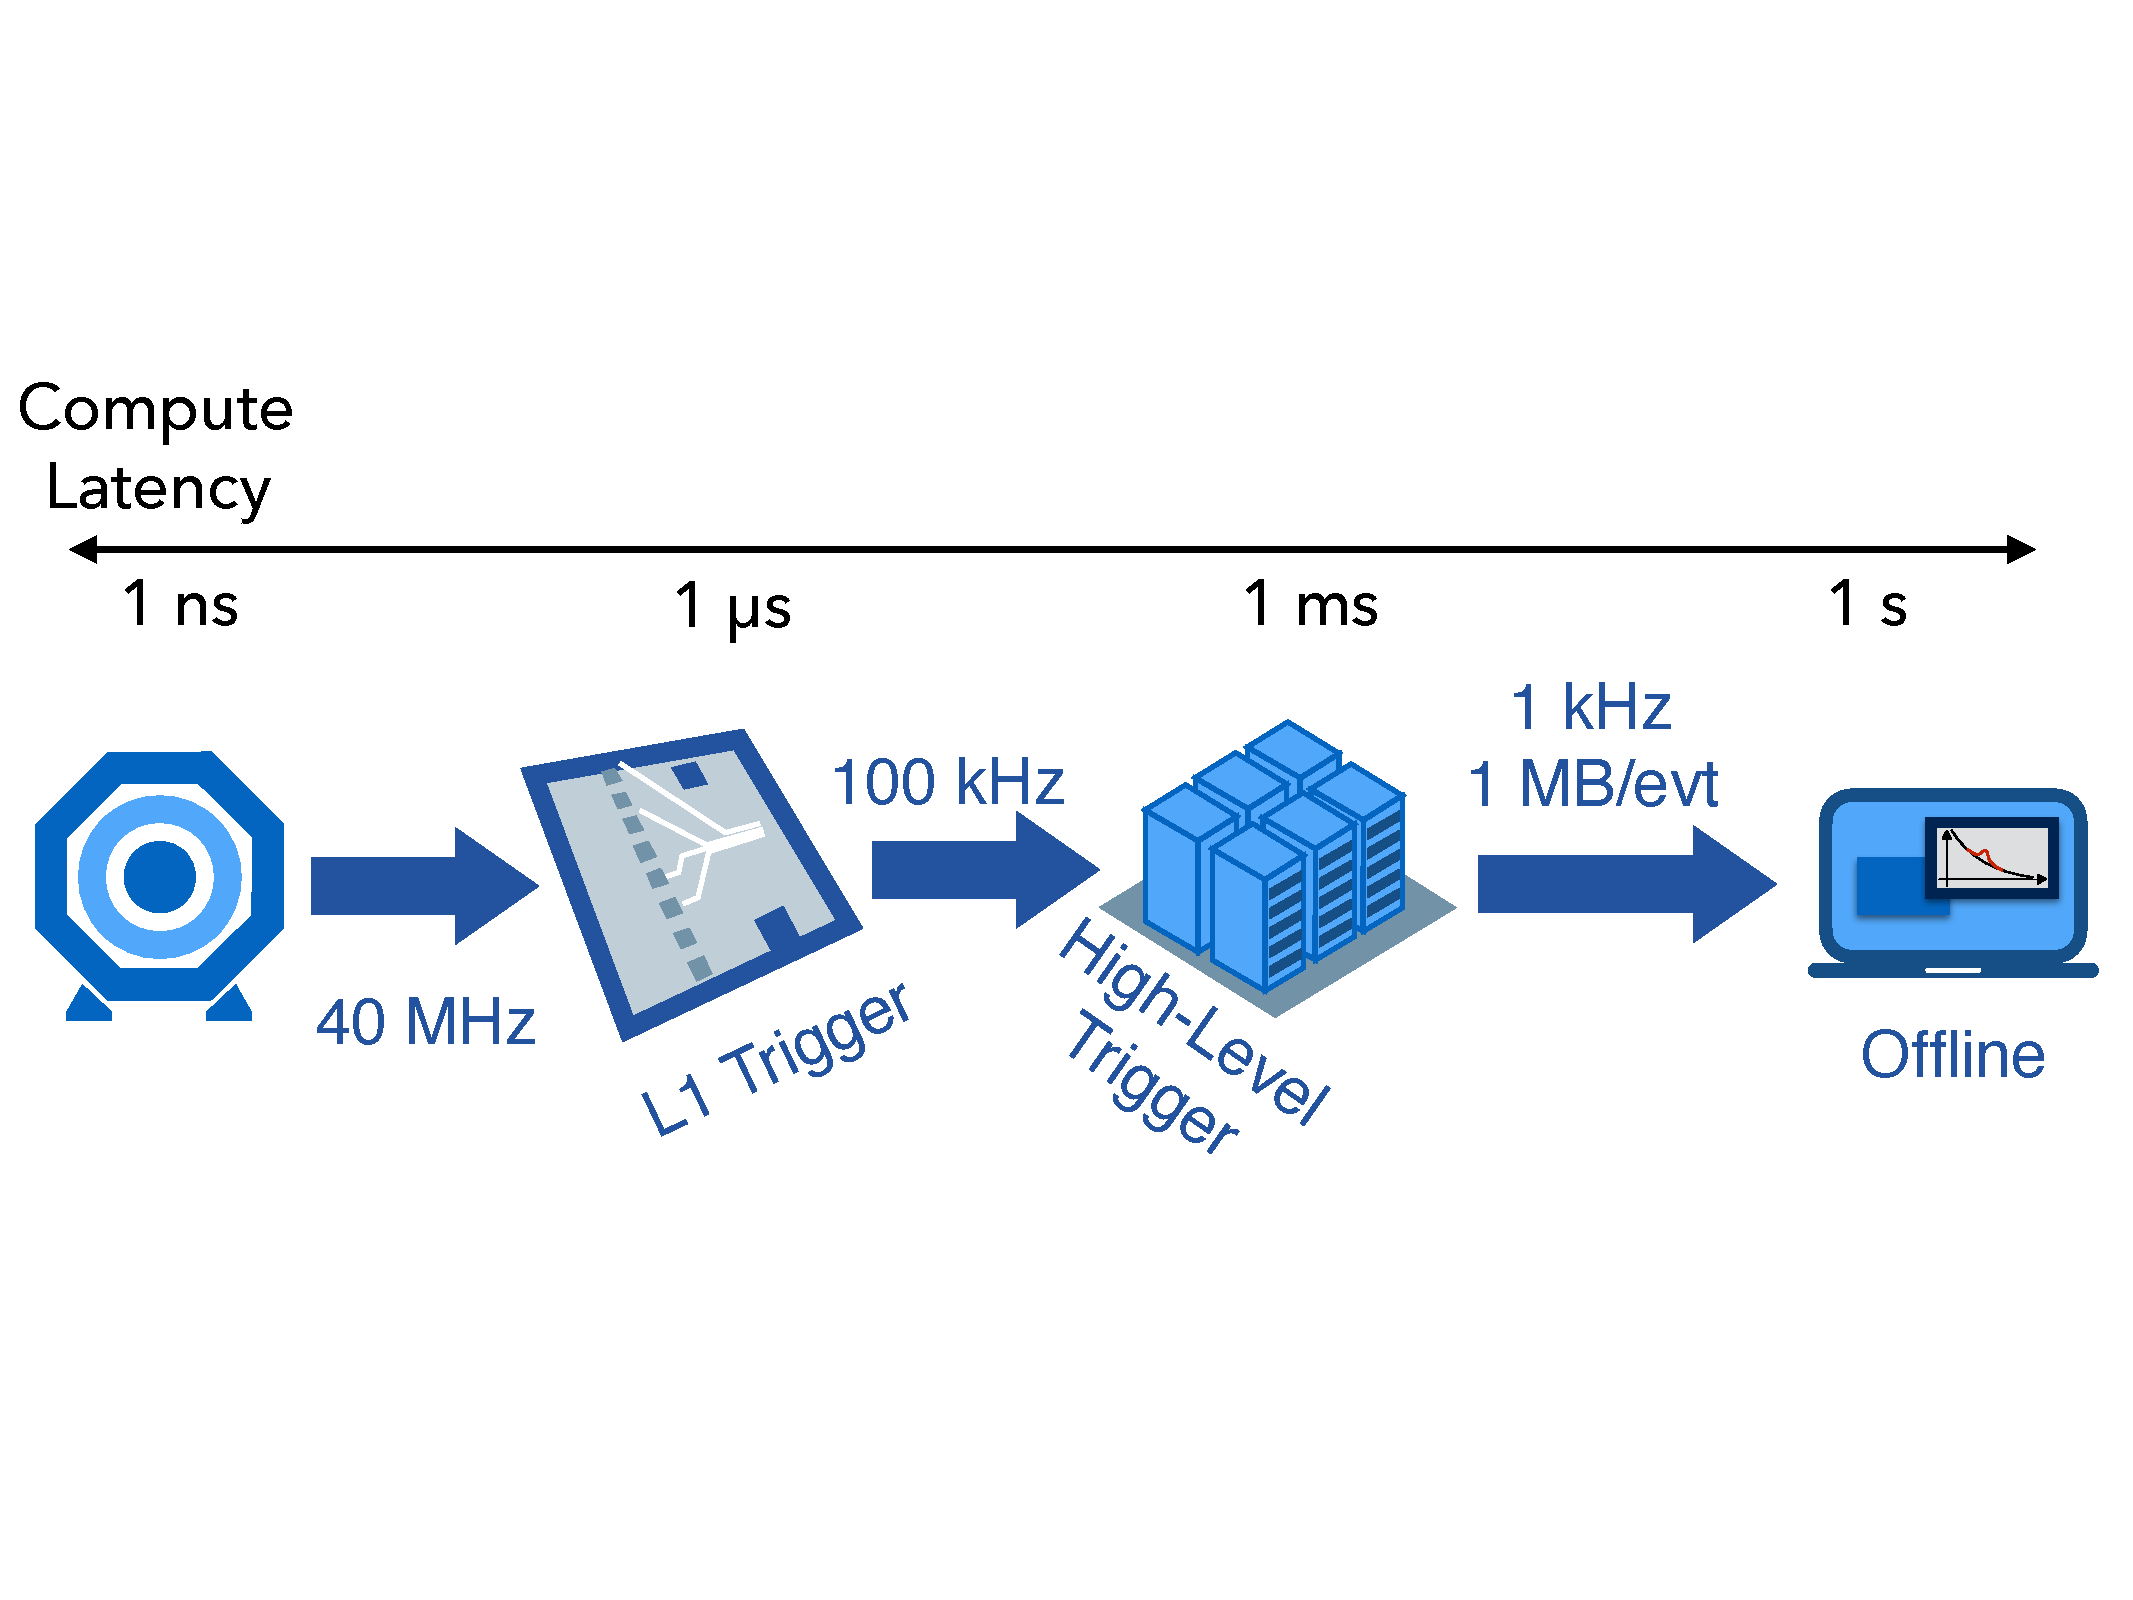
\includegraphics[viewport=0 200 1024 600, clip=true,width=\linewidth]{figures/cms_dataflow.pdf}
                  \end{center}
                  \begin{itemize}
                  \item Role of Trigger: Detect events that contains interesting data (decays of $\tau$s into 3 $\mu$s in our case).
                  \item We keep those events, and discard the uninteresting ones.
                    \item Machine Learning (ML) use case in particle physics: L1 Trigger, the first stage of real-time data processing and filtering
                     \item Due to low latency requirements, field programmable gate arrays (FPGAs) are used in Triggers
                    \item CERN CMS L1 Trigger requirements: high input data rates ($\approx40$ TB/s) into smaller output data rates ($\approx0.75$ TB/s), 
                    with fixed algorithm latency in the order of tens of nanoseconds.
                    \item High Level Synthesis (HLS) Compiler named \hlsfml~ is used to rapidly prototype ML models in FPGAs
              \end{itemize}
            \end{block}
            
            \begin{block}{Quest for Observing $\tau \rightarrow 3 \mu$}
                  \begin{itemize}
                  \item Decays of $\tau$ into 3 $\mu$ is predicted to be extremely rare in the Standard Model of particles physics.
                  \item New physical phenomena could enhance the probability significantly.
                  \item Observing these decays at the LHC could be a sign of the existence of physics beyond the standard model
              \end{itemize}
            \end{block}

            \begin{block}{Usage of Graph Neural Networks (GNN) in Filtering Task}
              \begin{itemize}
              \item Proton-proton collisions give data that can easily be formed as a graph.
              \item Graphs can easily connect the signals particles leave while traversing the CMS detector.
              \item Ideal for GNN, a Neural Network (NN) type that is optimized for graph based data (permutation invariant data).
              \item Good for $\mu$ detection from $\tau$ decay, as they have low transverse momentum ($p_t$) signature that makes
               it difficult for conventional ML Trigger algorithms to perform well.
                \end{itemize}
              \begin{columns}              
              \begin{column}{.49\textwidth}
                \begin{itemize}
              \item Task: Classification of events as Signal or Background in real-time using GNN.
              \item Performance quantified in a receiver operating
                characteristic (ROC) curve of signal efficiency versus
                Trigger Rate (kHz).
              \end{itemize}
            \end{column}
            \begin{column}{.49\textwidth}
             \begin{center}
                    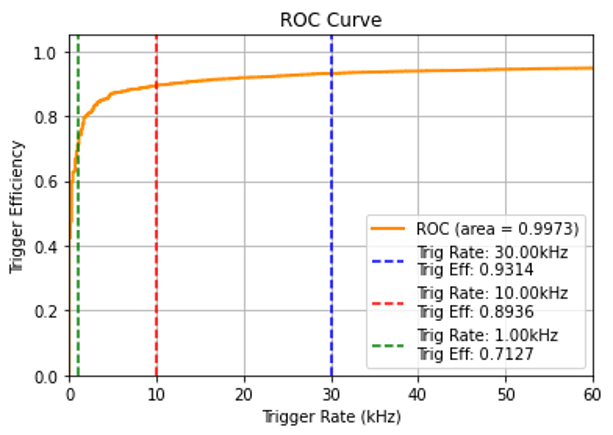
\includegraphics[width=\linewidth]{gnn_roc.png}
                  \end{center}
                \end{column}
                \end{columns}
              \end{block}
            
            \begin{block}{Summary}
                  \begin{itemize}
                    \item \hlsfml: compiler based on HLS for porting
                      fully-connected NNs to an FPGA from
                      conventional training frameworks such as {\tt
                        Keras} and {\tt PyTorch}
                      \item Focus on real-time
                        event reconstruction and filtering at the LHC
                        in FPGAs, with many other applications to real-time detector systems in the physical
                        sciences 
                        \item  Implemented a GCN model in HLS code, but too much resources
                        \item In the progress of implementing QAT to optimize GNN for low bit, low latency inference
                          \end{itemize}
                          \begin{flushright}\vspace{-3ex}
                           % \href{https://ml4physicalsciences.github.io/files/NeurIPS_ML4PS_2019_74.pdf}{
\includegraphics[width=0.18\textwidth]{qrcode.png}}
                          \end{flushright}
                  \end{block}  
              
                }
              \end{minipage}
            \end{beamercolorbox}
          \end{column}
    % ---------------------------------------------------------%
    % end the column

    % ---------------------------------------------------------%
    % Set up a column 
    \begin{column}{.49\textwidth}
      \begin{beamercolorbox}[center,wd=\textwidth]{postercolumn}
        \begin{minipage}[T]{.95\textwidth} 
          \parbox[t][\columnheight]{\textwidth}{
            
            \begin{block}{GNN Design}
                  \begin{center}
                    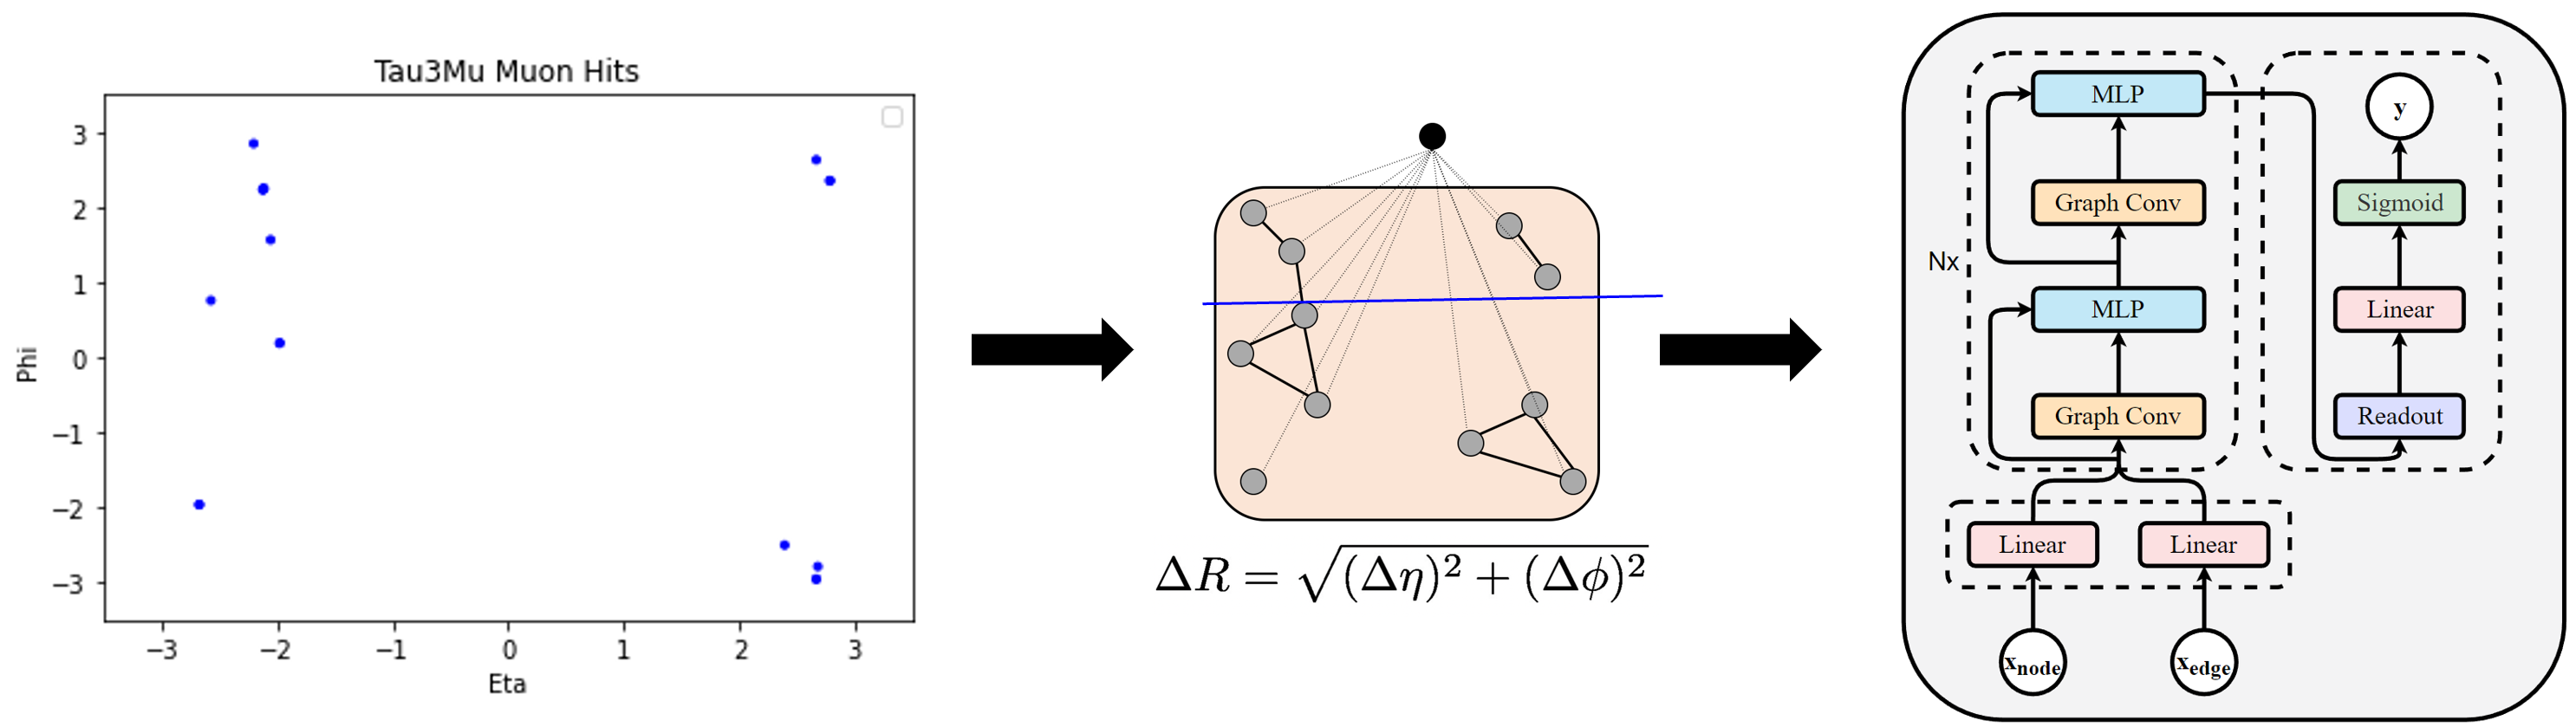
\includegraphics[width=\linewidth]{figures/graph_creation.png}
                  \end{center}
                \vspace{0.5in}
                \textbf{Graph Building}
                \begin{itemize}
                \item \textbf{Nodes Designation:} hits from Station 1 endcap detectors from CMS
                \item \textbf{Edge Designation:} edge between two nodes if $dR = \sqrt{\Delta \eta^2 + \Delta \phi^2} < 1$
                \item \textbf{Node features:} z and $\eta$ coordinate, and bend angle
                \item \textbf{Edge features:} $\Delta$z, $\Delta \eta$, $\Delta \phi$ and bend angle difference.
                \item Bend Angle: Angular difference of particles between hit signatures as they enter and exit the detector.
                \end{itemize}
                \vspace{0.2in}
                \textbf{GNN Architecture}
                \begin{itemize}
                \item \textbf{Type:} 8 Graph Convolution (GCN) Layers with residual connections in-between the layers.
                \item \textbf{MLP block:} 128 $\rightarrow$ 256 $\rightarrow$ 128 node fully-connected layers
                \end{itemize}
              \end{block}
            
            \begin{block}{FPGA Implementation via hls4ml}
             \begin{center}
                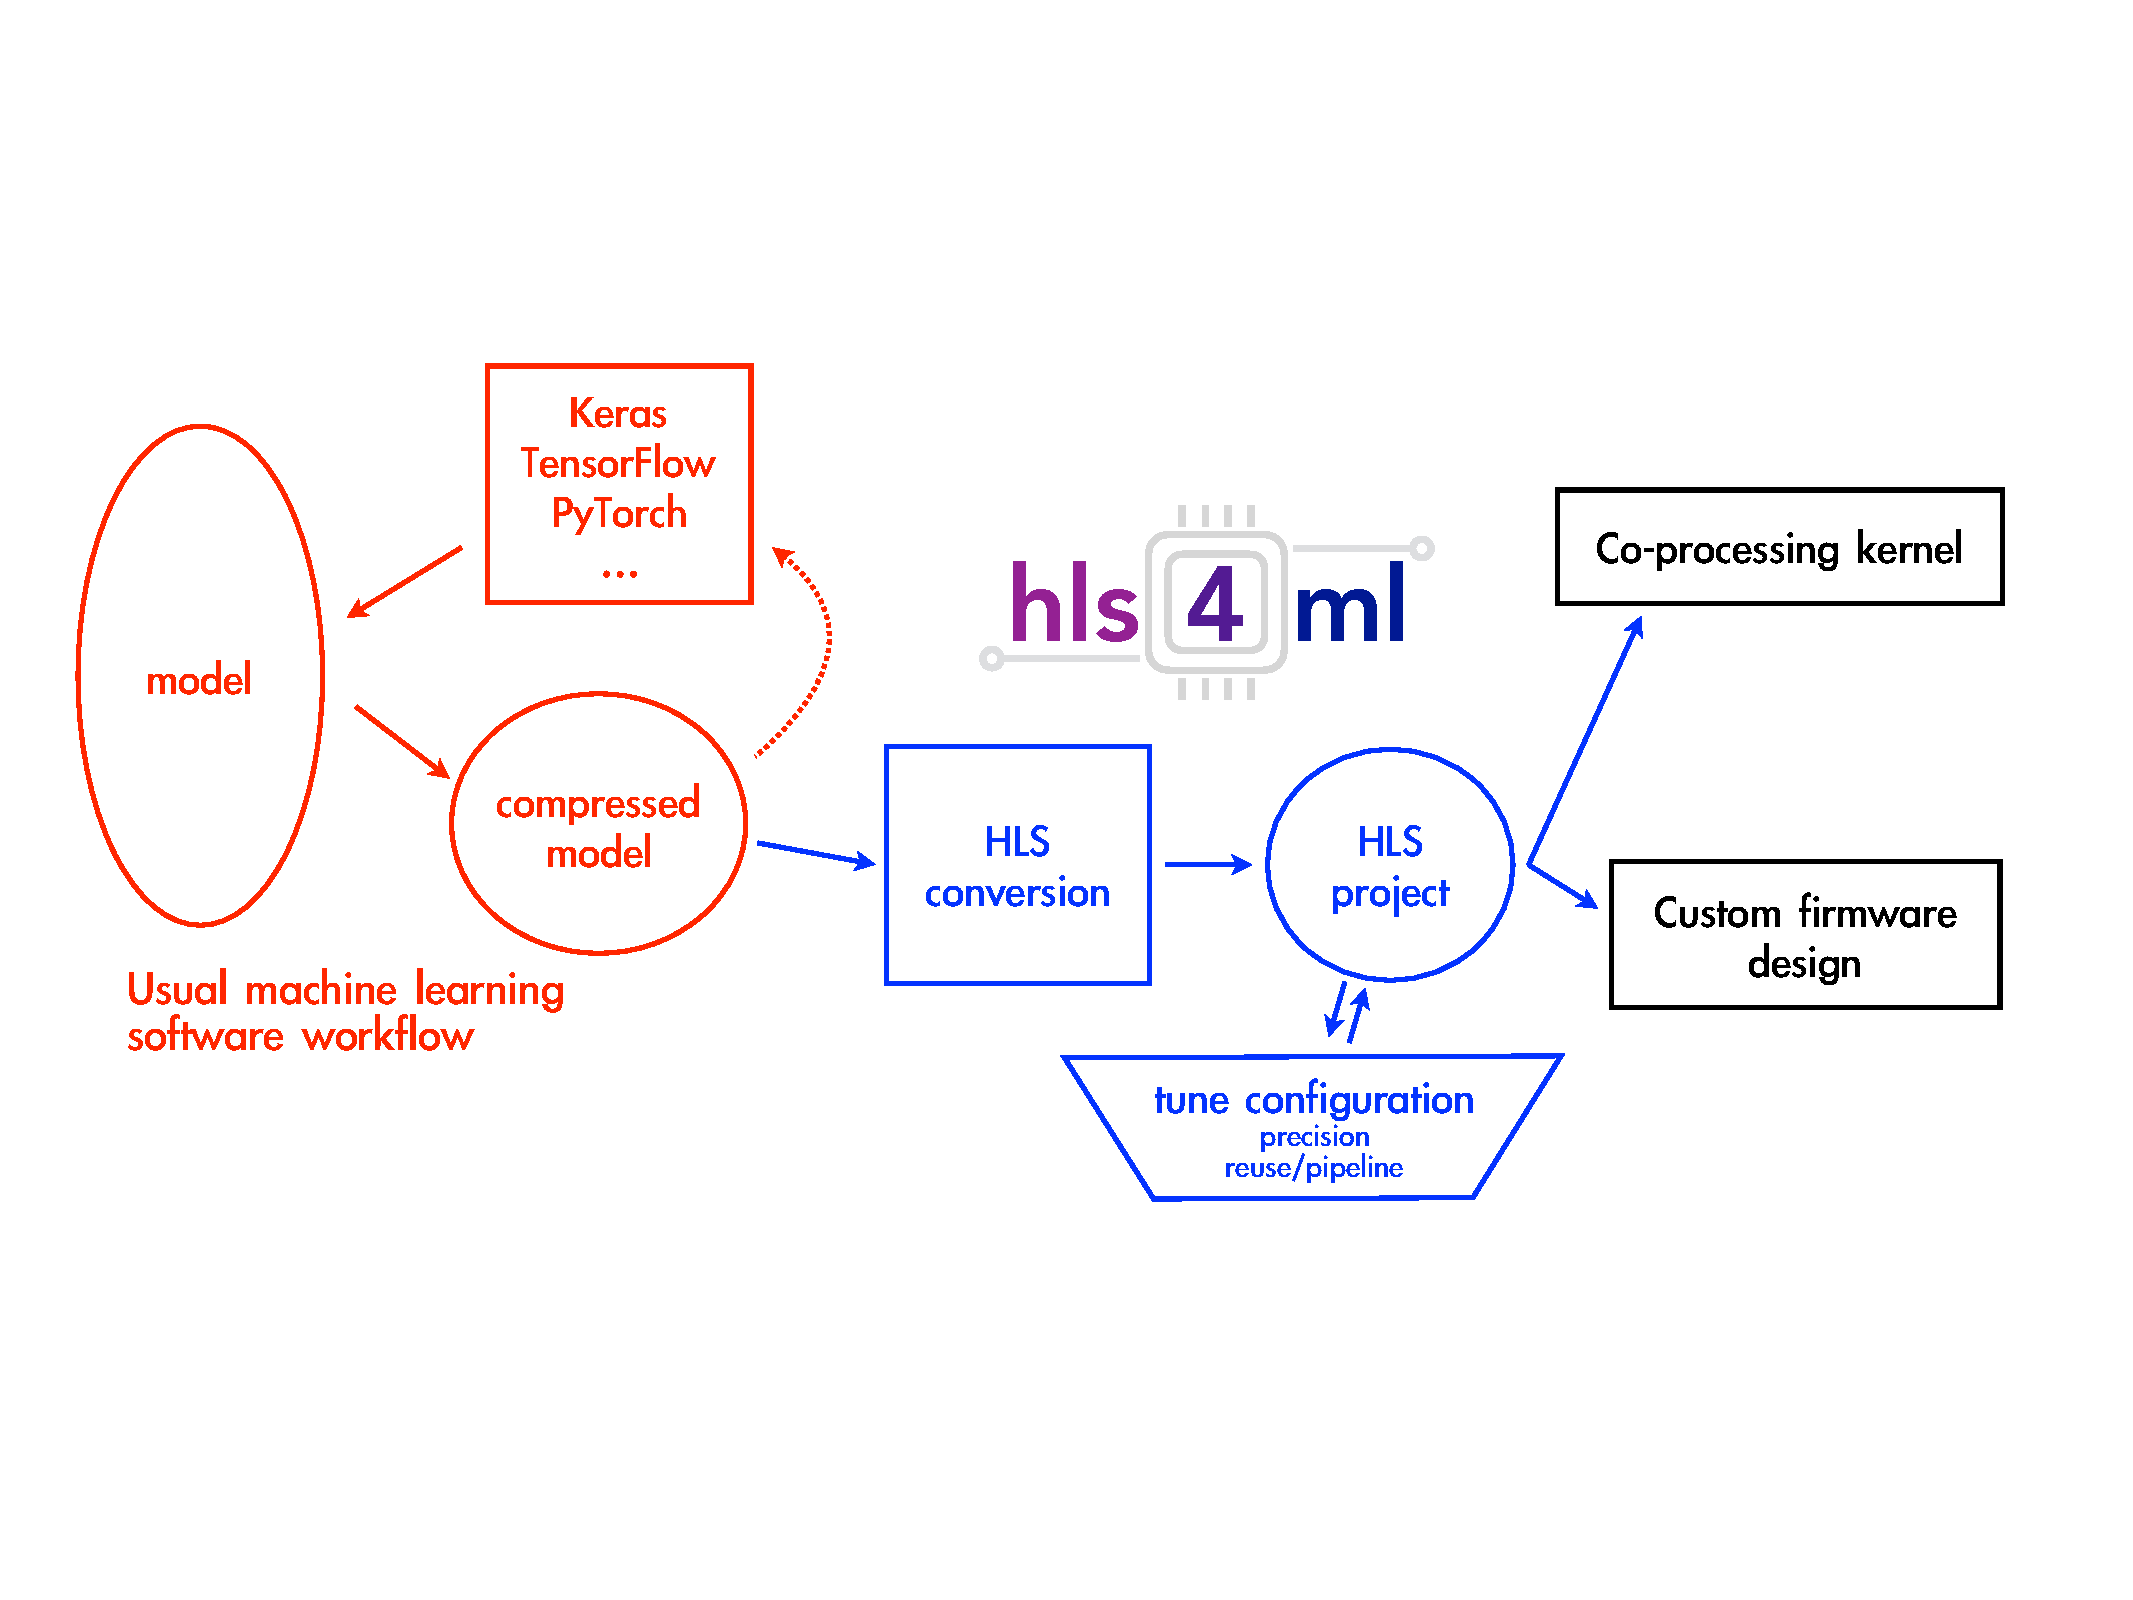
\includegraphics[width=0.8\linewidth]{flow-hls4ml.pdf}
              \end{center}
              \begin{itemize}
              \item \hlsfml\;is a pythonic compiler that translates  {\tt Keras} or {\tt PyTorch} NN models into High Level Synthesis (HLS) code.
              \item HLS ports said NN models to FPGAs for L1 Trigger.
               \item \hlsfml\;supports normal fully-connected NNs, but little GNN support.
                \item We have custom hard-coded our GNN model into \hlsfml, but FPGA resources overloaded. Our GNN model needs to be more lightweight
              \end{itemize}
             
            \end{block}
                  \begin{block}{Quantization Aware Training (QAT)}
                    Quantization of GNN is necessary to meet the FPGA latency constraints
                    \begin{itemize}
                    \item Typical NNs have their trainable parameters represented in a 32-bit system.
                    \item Quantization decreases the 32-bit representation to a more manageable number, typically 4 or 8 bits. 
                    \item \hlsfml \; uses arbituary precision fixed (ap-fixed) quantization method for faster inference.
                    \item Simply quantizing our pre-trained GNN greatly decreases performance.
                    \item QAT is a specialized method of training NNs that maintains performance with quantization.
                    \item Using {\tt Brevitas}, we demonstrated QAT on fully-connected NN with non $\tau \rightarrow 3 \mu$ data, for benchmarking.
                    \end{itemize}
                \vspace{0.5in}
                    To demonstrate QAT, we use Higgs Kaggle data as a benchmark (https://www.kaggle.com/competitions/higgs-boson/data)
                   \begin{center}
                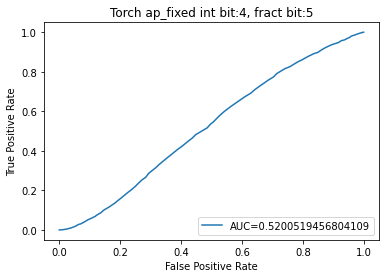
\includegraphics[width=0.49\linewidth]{figures/torch_quantized.png}
                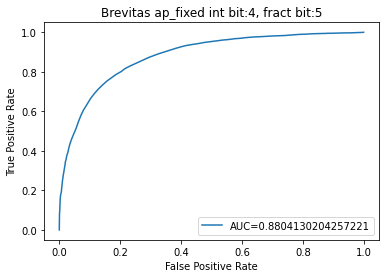
\includegraphics[width=0.49\linewidth]{figures/bv_quantized.png}
              \end{center}
                  
                \end{block}                
                                
          }
          % ---------------------------------------------------------%
          % end the column
        \end{minipage}
      \end{beamercolorbox}
    \end{column}
    % ---------------------------------------------------------%
    % end the column
  \end{columns}
  \vskip1ex
  %\tiny\hfill\textcolor{ta2gray}{Created with \LaTeX \texttt{beamerposter}  \url{http://www-i6.informatik.rwth-aachen.de/~dreuw/latexbeamerposter.php}}
  %\tiny\hfill{Created with \LaTeX \texttt{beamerposter}  \url{http://www-i6.informatik.rwth-aachen.de/~dreuw/latexbeamerposter.php} \hskip1em}
\end{frame}
\end{document}


%%%%%%%%%%%%%%%%%%%%%%%%%%%%%%%%%%%%%%%%%%%%%%%%%%%%%%%%%%%%%%%%%%%%%%%%%%%%%%%%%%%%%%%%%%%%%%%%%%%%
%%% Local Variables: 
%%% mode: latex
%%% TeX-PDF-mode: t
%%% Comments below:



\href{https://jduarte.physics.ucsd.edu}{Javier Duarte}{\color{lightgray}\inst{1,2}},  Christian Herwig{\color{lightgray}\inst{2}},
	  Burt Holzman{\color{lightgray}\inst{2}}, Sergo Jindariani{\color{lightgray}\inst{2}}, Benjamin
	  Kreis{\color{lightgray}\inst{2}},  \href{https://mia.physics.purdue.edu/}{Mia Liu}{\color{lightgray}\inst{2}}, Ryan
	  Rivera{\color{lightgray}\inst{2}},  Nhan Tran{\color{lightgray}\inst{2}},  Song Han{\color{lightgray}\inst{3}},  Phil
	  Harris{\color{lightgray}\inst{3}},  Dylan Rankin{\color{lightgray}\inst{3}}, Vladimir Loncar{\color{lightgray}\inst{4}},
	  Jennifer Ngadiuba{\color{lightgray}\inst{4}}, Maurizio Pierini{\color{lightgray}\inst{4}}, Sioni
	  Summers{\color{lightgray}\inst{4}}, Scott Hauck{\color{lightgray}\inst{5}}, Shih-Chieh Hsu{\color{lightgray}\inst{5}}, Zhenbin Wu{\color{lightgray}\inst{6}},  Edward 	Kreinar{\color{lightgray}\inst{7}}
	  
	  
	   \begin{itemize}
                \item {\bf compression}, the three-hidden-layer model with 70\% of the parameters removed using iterative retraining with $L_1$ regularization and magnitude-based pruning
                \item {\bf quantization}, the precision of the inputs, weights, and biases
                \item {\bf parallelization}, the number of times a
                  given multiplier is used for a layer computation,
                  quantified by a \emph{reuse factor}
                \end{itemize}
                \vspace{0.5in}
                With these handles, monitor 
                \begin{itemize}
                \item {\bf resources}: digital signal processors
                  (DSPs), block random access memory (BRAM), flip-flops (FFs), and lookup tables (LUTs)
                \item {\bf latency}: time it takes to compute the full network
                \item {\bf initiation interval (II)}: time before a new set of inputs can be accepted
                \end{itemize}
                
 To enhance the flexibility of \hlsfml, several new
                    developments include
                    \begin{itemize}
                    \item extension to allow for
                      significantly larger dense networks in terms of the number of neurons per layer
                    \item inclusion of zero-suppression for weights
                      stored in on-chip memory or BRAM, reducing the use of on-chip logic registers
                    \item addition of binary and ternary matrix multiplication
                    \end{itemize}
                \vspace{0.5in}
                    To demonstrate the new developments, several versions of a large dense network to classify handwritten MNIST digits are benchmarked
                    \begin{center}
                    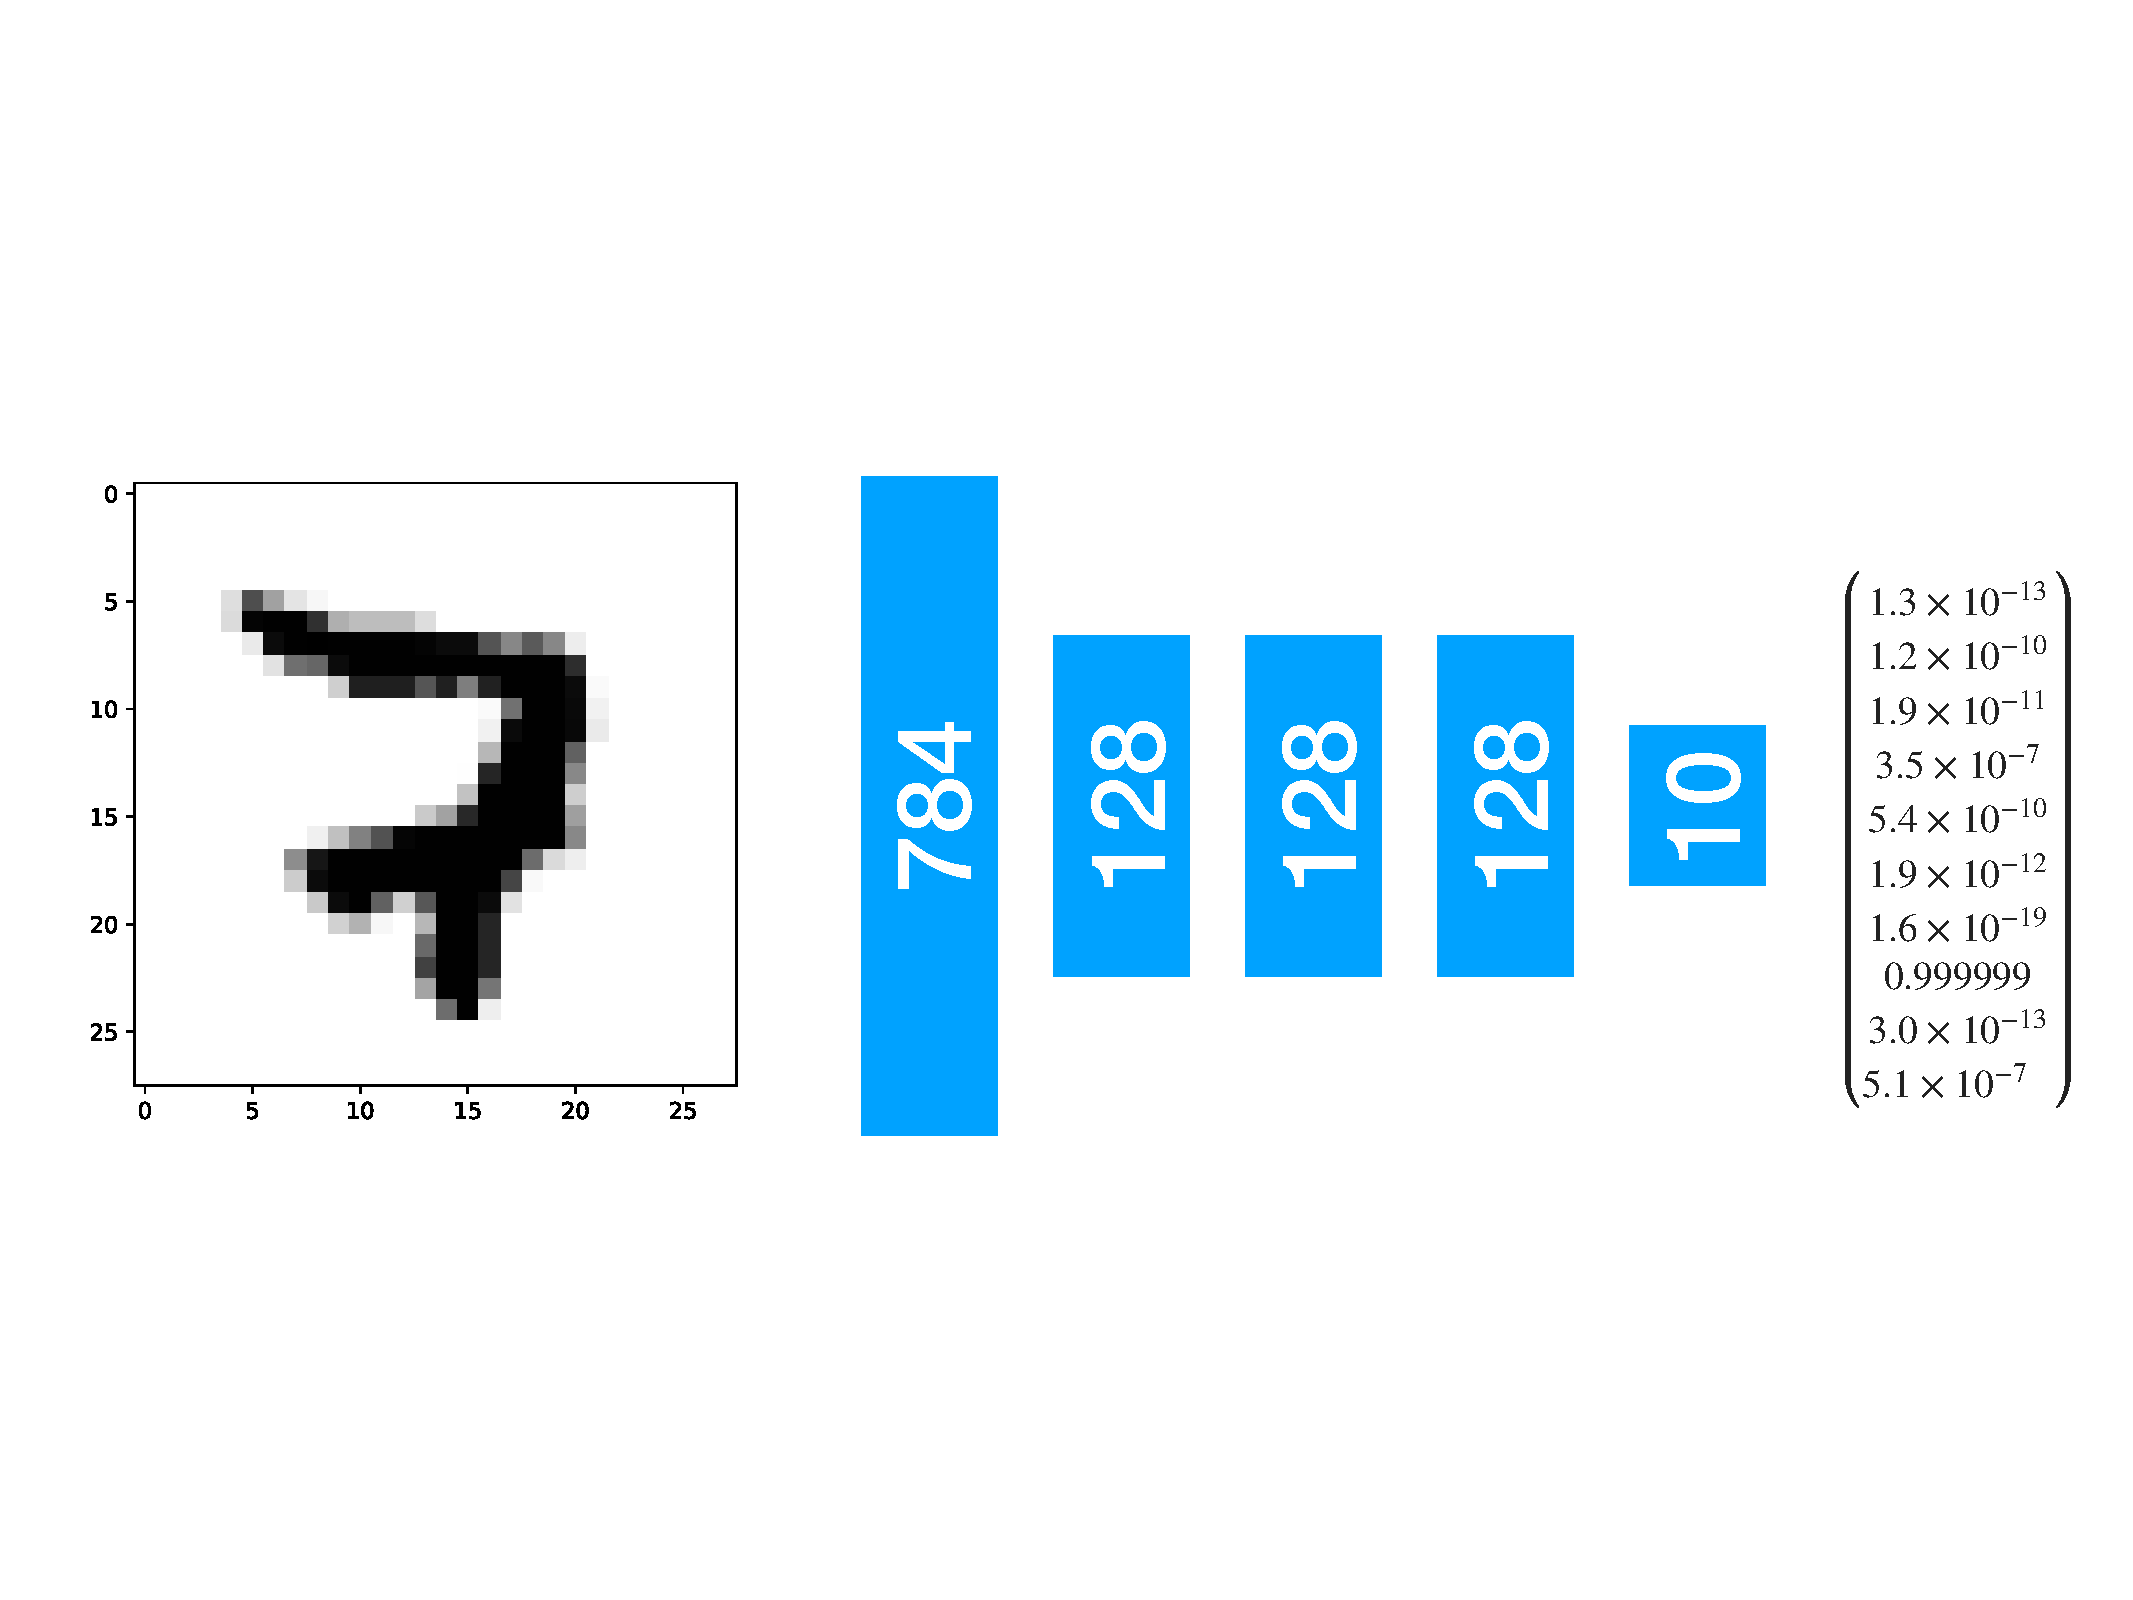
\includegraphics[width=\linewidth]{MNIST_big.pdf}
                  \end{center}
                  \begin{center}
                    \resizebox{\textwidth}{!}{
                      \begin{tabular}{l|ccccccc}
                        \textbf{Model} & \textbf{II} & \textbf{Accuracy} &\textbf{Latency} & \textbf{DSP}  & \textbf{BRAM} & \textbf{FF}  & \textbf{LUT}\\\hline
                        MNIST dense                                            &  128 & 0.97 & 2.6~$\mu$s & 21\% & 45\%& 12\% & 33\%\\
                        MNIST binary dense                                 &  128 & 0.93 & 2.6~$\mu$s & 0\% & 33\%& 7\% & 39\%\\ 
                        MNIST ternary dense                                &  128 & 0.95 & 2.6~$\mu$s & 0\% & 33\%& 7\% & 40\%\\ 
                        MNIST dense, 95\% pruned &  128 & 0.96 & 2.8~$\mu$s & 1\% & 34\% & 13\% & 164\%\\
                        MNIST dense                       &  4096 & 0.97 & 68.1~$\mu$s &1\% & 66\%&27\% &83\%\\ 
                        MNIST dense, 95\% pruned &  4096 & 0.96 & 82.1~$\mu$s & 0\% & 34\% & 9\% & 25\%\\ 
                      \end{tabular}}  
